%\input{../data/cameraPose.txt}
%\input{../data/errorPose.txt}
\input{../data/errorPoseX.txt}

%Time Plot
% \newcommand{\cameraPosePlot}{
% \label{plo:cameraPosePlot}
% \begin{figure}[!ht]
% \centering
% 	\begin{tikzpicture}
% 		\begin{axis}[height=9cm, width=\textwidth, grid=major,xlabel={Step},ylabel={Time[s]}]
			
% 			\addplot [color=SkyBlue, mark=o] coordinates {
% 				\cameraPose
% 			};
% 			\addlegendentry{t}

% 		\end{axis}
% 	\end{tikzpicture}
% \end{figure}
% }

\newcommand{\qRobotPlot}{
\label{plo:qRobotPlot}
\begin{figure}[!ht]
\centering
	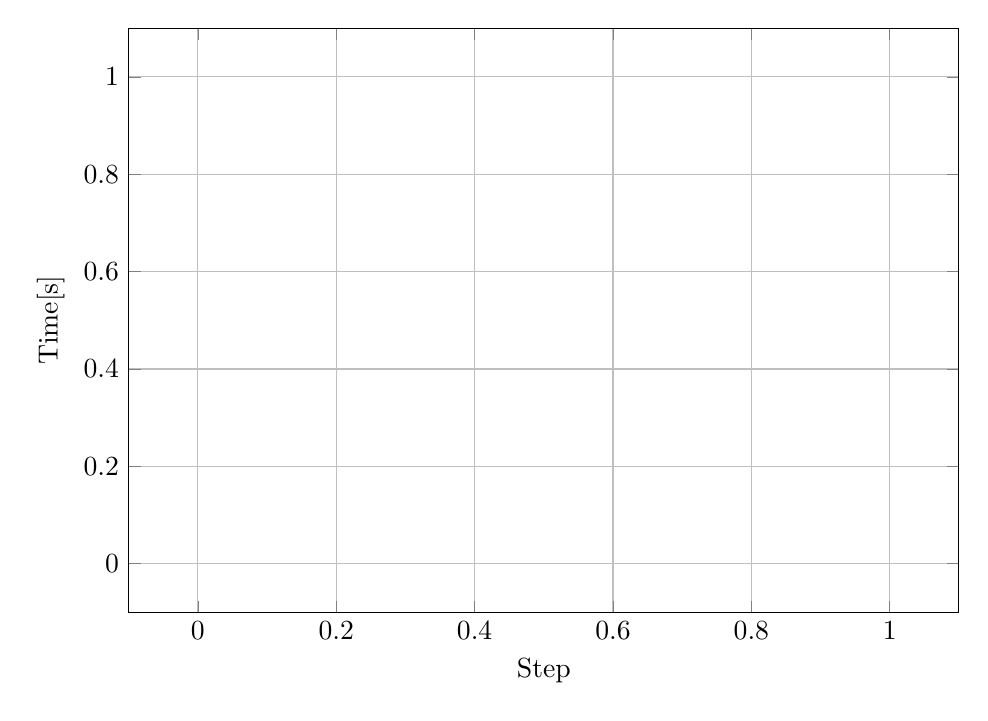
\begin{tikzpicture}
		\begin{axis}[height=9cm, width=\textwidth, grid=major,xlabel={Step},ylabel={Time[s]}]
			
			\addplot [color=SkyBlue, mark=o] coordinates {
				\errorPoseDataX
			};
			\addlegendentry{t}

		\end{axis}
	\end{tikzpicture}
\end{figure}
}